\documentclass[aspectratio=169]{beamer}
\usepackage{pgf}
\usepackage{multimedia}
\usepackage{colortbl,tabularx,mathrsfs,calligra,xcolor}
\usepackage{amsmath,amsfonts,amssymb,amsthm}
\usepackage{ragged2e}
\usepackage{setspace}
\usepackage{filecontents}
\usepackage{caption}
\usepackage{subcaption}
\usepackage{contour}
\usepackage{fancybox}
\usepackage{wrapfig}
\usepackage{multirow}
\usepackage{multicol}
\usepackage{pgfplots, tkz-euclide,calc}
    \usetikzlibrary{patterns,snakes,shapes.arrows,shapes.geometric,arrows}
\usepackage{listings}
\usepackage{enumitem}
\usepackage{pifont}
\usepackage[scaled]{berasans}
    \renewcommand*\familydefault{\sfdefault}  %% Only if the base font of the document is to be sans serif
\usepackage[T1]{fontenc}
\usepackage{hyperref}
\hypersetup{
    filecolor=magenta,      
    urlcolor=cyan,
    pdftitle={Overleaf Example},
    pdfpagemode=FullScreen,
    }
\renewcommand*\familydefault{\sfdefault} %% Only if the base font of the document is to be sans serif

\graphicspath{{C:/Users/teoso/OneDrive/Documents/Asisten Dosen & Lab/Asisten Laboratorium/Alpro 1/PPT/Graphicx/}}

\definecolor{HIMAmuda}{HTML}{01D1FD}
\definecolor{HIMAtua}{HTML}{02016A}
\definecolor{HIMAabu}{HTML}{CBCBCC}
\definecolor{PastelGreen}{HTML}{77DD77}
\definecolor{pgray}{rgb}{0.5,0.5,0.5}
\definecolor{pblue}{rgb}{0.13,0.13,1}
\definecolor{pgreen}{rgb}{0,0.5,0}
\definecolor{pred}{rgb}{0.9,0,0}
\definecolor{pgrey}{rgb}{0.46,0.45,0.48}
\definecolor{pcyan}{HTML}{D4EFFC}
\definecolor{lblue}{HTML}{00AEEF}
\definecolor{input}{HTML}{AAE1FA}
\definecolor{bg}{rgb}{0.95, 0.95, 0.92}
\definecolor{vscode}{HTML}{282A36}

\usetheme{Madrid}

\setbeamercolor{palette primary}{bg=HIMAtua,fg=white}
\setbeamercolor{palette secondary}{bg=HIMAmuda,fg=black}
\setbeamercolor{palette tertiary}{bg=HIMAabu,fg=black}
\setbeamercolor{palette quaternary}{bg=HIMAmuda,fg=white}
\setbeamercolor{structure}{fg=HIMAmuda} % itemize, enumerate, etc
\setbeamercolor{section in toc}{fg=HIMAtua} % TOC sections
\setbeamercolor{block title alerted}{fg=white,bg=magenta}
\setbeamercolor{block body alerted}{fg=black!90,bg=pink}

\usefonttheme{professionalfonts}
\setbeamertemplate{theorems}[numbered]
\setbeamertemplate{itemize items}[circle]

\usebackgroundtemplate{%
\tikz[overlay,remember picture] \node[opacity=0.1, at=(current page.center)]{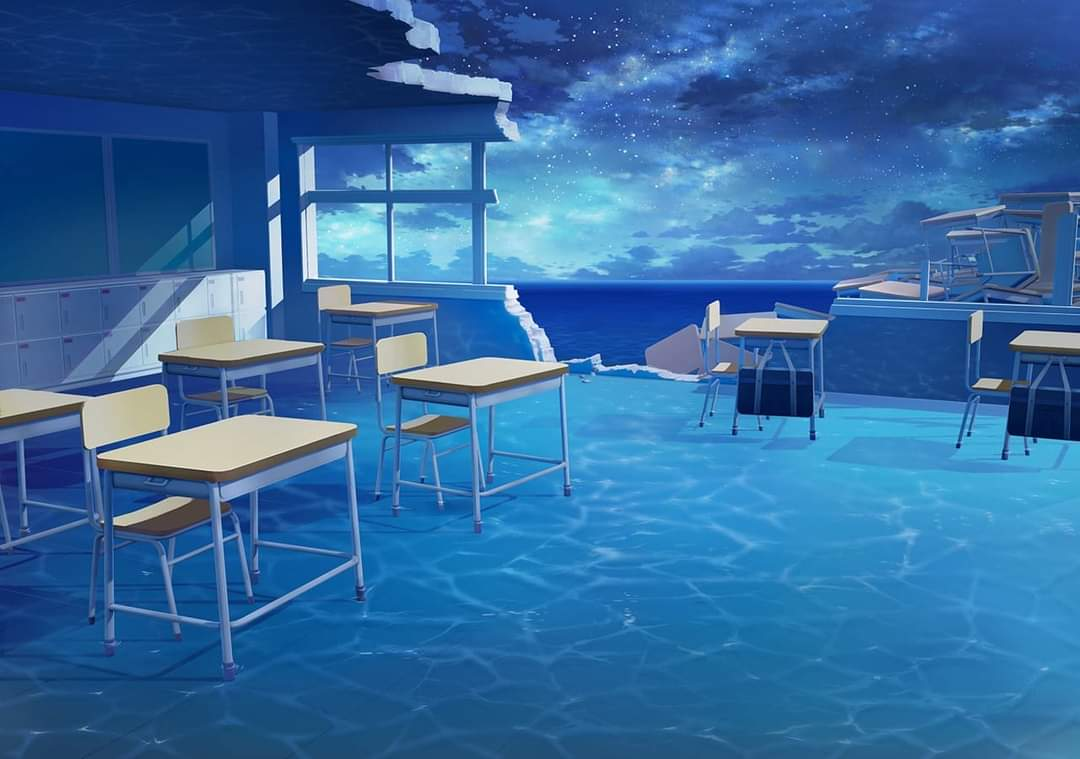
\includegraphics[width=\paperwidth]{plana class}};
}

\renewcommand\thesubfigure{\arabic{subfigure}}
\newtheorem*{funfact}{Fun Fact}
\newtheorem{latihan}{Latihan}
\newtheorem*{definisi}{Definisi}
\newtheorem{teorema}{Teorema}
\theoremstyle{definition}
\newtheorem*{contoh}{Contoh}
\newtheorem*{masalah}{Masalah}
\newcommand{\R}{\mathbb{R}}

\AtBeginEnvironment{contoh}{%
    \setbeamercolor{block title}{use=example text,fg=white,bg=example text.fg!75!black}
    \setbeamercolor{block body}{parent=normal text,use=block title example,bg=block title example.bg!10!bg}
}

\AtBeginEnvironment{funfact}{%
  \setbeamercolor{block title}{fg=white,bg=PastelGreen!50!HIMAmuda} % Set title background to pastel green and text to white
  \setbeamercolor{block body}{parent=normal text,bg=PastelGreen!50!HIMAmuda!30!white} % Set body background to a lighter pastel green
}
\AtBeginEnvironment{definisi}{
    \setbeamercolor{block title}{fg=white,bg=HIMAtua}
    \setbeamercolor{block body}{parent=normal text,bg=HIMAtua!30!white}
}
\AtBeginEnvironment{teorema}{
    \setbeamercolor{block title}{bg=darkgray,fg=white}
    \setbeamercolor{block body}{parent=pallette tertiary,bg=HIMAabu!30!white}
}
\AtBeginEnvironment{latihan}{%
  \setbeamercolor{block title}{fg=white,bg=PastelGreen} % Set title background to pastel green and text to white
  \setbeamercolor{block body}{parent=normal text,bg=PastelGreen!30!white} % Set body background to a lighter pastel green
}
\AtBeginEnvironment{masalah}{%
  \setbeamercolor{block title}{fg=white,bg=teal} % Set title background to pastel green and text to white
  \setbeamercolor{block body}{parent=normal text,bg=teal!30!white} % Set body background to a lighter pastel green
}

\renewcommand{\arraystretch}{1.3}

\usepackage{listings}

\lstdefinestyle{standard}{
    language            = Java,
    showspaces          = false,
    showtabs            = false,
    breaklines          = true,
    showstringspaces    = false,
    breakatwhitespace   = true,
    commentstyle        = \color{pgray},
    keywordstyle        = \color{pblue},
    stringstyle         = \color{pgreen},
    basicstyle          = \footnotesize\ttfamily,
    frame               = shadowbox,
    backgroundcolor     = \color{brown!10!white},
    escapeinside        = {(*}{*)},
    numbers             = left, % {none, left, right}
    numberstyle         = \scriptsize\color{lightgray},
    numbersep           = -8pt,
    rulesepcolor        =\color{brown!50!black}
    }

\lstdefinestyle{output}{
    language=Java,
    backgroundcolor     =\color{vscode},
    basicstyle          =\footnotesize\ttfamily\color{white},
    frame               =shadowbox,
    escapeinside        ={(*}{*)},
    showspaces          =false,
    showtabs            =false,
    breaklines          =true,
    showstringspaces    =false,
    breakatwhitespace   =true,
    rulesepcolor        =\color{HIMAtua!50!white},
    rulecolor           =\color{HIMAtua!50!white},
    numbers             =none,
    }

\lstset{style=standard}

\tikzstyle{startstop} = [rectangle, rounded corners, 
minimum width=2cm, 
minimum height=1cm,
text centered, 
draw=black, 
fill=pink]

\tikzstyle{io} = [trapezium, 
trapezium stretches=true, % A later addition
trapezium left angle=70, 
trapezium right angle=110, 
minimum width=2cm, 
minimum height=1cm, text centered, 
draw=black, fill=HIMAmuda]

\tikzstyle{process} = [rectangle, 
minimum width=2cm, 
minimum height=1cm, 
text centered, 
text width=2cm, 
draw=black, 
fill=HIMAabu]

\tikzstyle{decision} = [diamond, 
minimum width=2cm, 
minimum height=1cm, 
text centered, 
draw=black, 
fill=PastelGreen]
\tikzstyle{arrow} = [thick,->,>=stealth]

\newcommand{\enter}{\raisebox{-1.8pt}{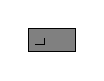
\begin{tikzpicture}[scale=0.3]
    \draw[thin,fill=gray] (0,0) rectangle (2,1);
    \draw (0.3,0.3) -- (0.7,0.3)--(0.7,0.6);     
\end{tikzpicture}}}

\newcommand{\inputscan}[1]{\raisebox{0pt}[1pt]{\colorbox{darkgray}{#1}}}

\author[Tew \& Haf]{Hafidz Mulia\\Teosofi Hidayah Agung}
\date{7 Oktober 2024}
\title[Alpro 1 - Week 5]{Looping}
\institute[Matematika ITS]{Departemen Matematika\\ Institut Teknologi Sepuluh Nopember}
\titlegraphic{{
\includegraphics[scale=0.02]{M.png}$\quad$
\includegraphics[scale=0.2]{Provicom.png}}}

\begin{document}
    {\usebackgroundtemplate{
        \tikz[overlay,remember picture] \node[opacity=0.2, at=(current page.center)]{
\includegraphics[width=\paperwidth]{bg_2}};}
    \begin{frame}
        \titlepage
    \end{frame}
    }

    \AtBeginSection{
    {\usebackgroundtemplate{
     \tikz[overlay,remember picture] \node[opacity=0.1, at=(current page.center)]{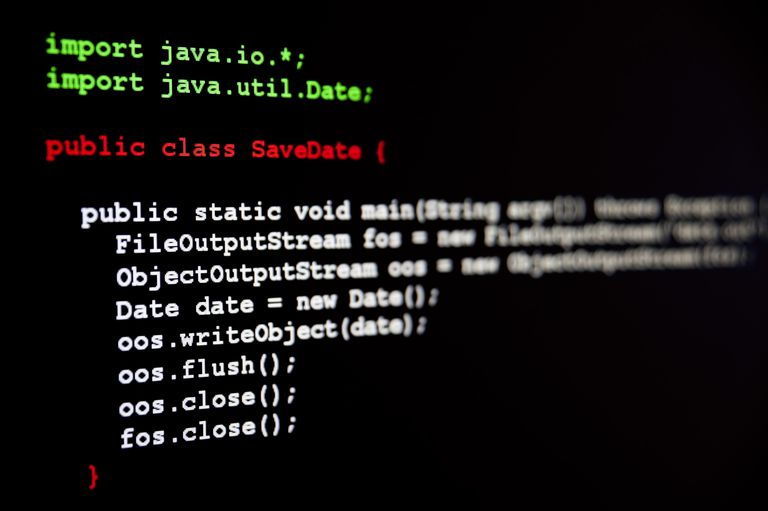
\includegraphics[width=\paperwidth]{Java code}};}
    \begin{frame}{Daftar isi}
        \tableofcontents[currentsection]
    \end{frame}}
    }

    {\usebackgroundtemplate{
     \tikz[overlay,remember picture] \node[opacity=0.1, at=(current page.center)]{
\includegraphics[width=\paperwidth]{jojo}};}
    \begin{frame}
        \begin{masalah}
            Melakukan sesuatu yang sama berulang kali adalah hal yang terkadang membosankan. Hal itu akan berakibat ketidakfokusan dalam prosesnya yang berujung pada kesalahan. Namun kita bisa tenang, karena komputer tidak memiliki sifat jenuh seperti manusia. Komputer dapat melalukan sesuatu berulang kali tanpa terjadinya kesalahan asalkan kita memberikan instruksi yang benar.
        \end{masalah}
    \end{frame}
    }

    \section{For}
    \begin{frame}[fragile]
        \frametitle{\insertsection}
        \begin{definisi}
            \textbf{For} adalah salah satu struktur pengulangan yang digunakan untuk melakukan sesuatu berulang kali. Struktur ini memiliki tiga bagian, yaitu inisialisasi, kondisi, dan increment/decrement. Struktur ini biasanya digunakan ketika kita mengetahui berapa kali kita akan melakukan sesuatu.
        \end{definisi}
        \begin{lstlisting}[caption={Syntax For}, numbers=none]
    for ("inisialisasi"; "kondisi"; "increment/decrement") {
        // Perintah yang akan diulang
    }
        \end{lstlisting}
    \end{frame}

    \begin{frame}
        \frametitle{\insertsection}
        \begin{figure}
            \centering
            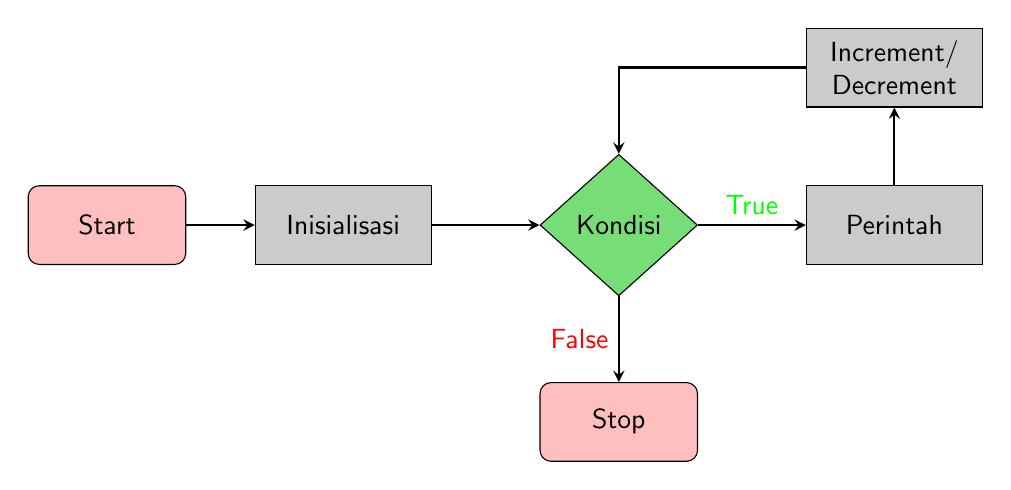
\begin{tikzpicture}
                \node (start) [startstop] {Start};
                \node (pro1) [process, right of=start, xshift=2cm] {Inisialisasi};
                \node (dec1) [decision, right of=pro1, xshift=2.5cm] {Kondisi};
                \node (pro2) [process, right of=dec1, xshift=2.5cm] {Perintah};
                \node (pro3) [process, above of=pro2, yshift=1cm] {Increment/\\Decrement};
                \node (stop) [startstop, below of=dec1, yshift=-1.5cm] {Stop};

                \draw [arrow] (start) -- (pro1);
                \draw [arrow] (pro1) -- (dec1);
                \draw [arrow] (dec1) -- node[anchor=south] {\color{green}True} (pro2);
                \draw [arrow] (dec1) -- node[anchor=east] {\color{red}False} (stop);
                \draw [arrow] (pro2) -- (pro3);
                \draw [arrow] (pro3) -| (dec1);
            \end{tikzpicture}
            \caption{Flowchart For}
        \end{figure}
    \end{frame}

    \begin{frame}[fragile]
        \frametitle{\insertsection}
        \begin{contoh}
            Menampilkan barisan aritmatika $-2, 1, 4, 7, \dots$ sebanyak 20 suku.
        \end{contoh}
        \begin{lstlisting}
    int suku_n = -2;
    for (int n = 1; n <= 20; n++) {
        System.out.print(suku_n+" ");
        suku_n += 3;
    }
        \end{lstlisting}
        \begin{lstlisting}[style=output]

    -2 1 4 7 10 13 16 19 22 25 28 31 34 37 40 43 46 49 52 55
(**)
        \end{lstlisting}
    \end{frame}

    \subsection{Nested}
    \begin{frame}[fragile]
        \frametitle{\insertsection}
        \framesubtitle{\insertsubsection}
        \begin{contoh}
            Membuat segitiga siku-siku dengan simbol \texttt{*} sebanyak 5 baris.
        \end{contoh}
        \begin{lstlisting}
    for (int i = 1; i <= 5; i++) {
        for (int j = 1; j <= i; j++) {
            System.out.print("*");
        }
        System.out.println();
    }
        \end{lstlisting}
        \begin{lstlisting}[style=output]
    *
    **
    ***
    ****
    *****
        \end{lstlisting}
    \end{frame}

    \begin{frame}[fragile]
        \frametitle{\insertsection}
        \begin{alertblock}{Infinite Loop}
            Berhati-hatilah ketika menggunakan loop, karena jika tidak memperhatikan kondisi yang diberikan, maka akan terjadi \textit{infinite loop} yang akan membuat program tidak berhenti hingga program mengalami \textit{Stack Overflow}.
        \end{alertblock}
        \begin{lstlisting}[caption={Infinite Loop},firstnumber=6]
    for (int i = 1; i <= 5; i--) {
        System.out.println(i);
    }
        \end{lstlisting}
    \end{frame}

    \section{While}
    \begin{frame}[fragile]
        \frametitle{\insertsection}
        \begin{definisi}
            \textbf{While} adalah salah satu struktur pengulangan yang digunakan untuk melakukan sesuatu berulang kali. Struktur ini hanya memiliki satu bagian, yaitu kondisi. Struktur ini biasanya digunakan ketika kita tidak mengetahui berapa kali kita akan melakukan sesuatu.
        \end{definisi}
        \begin{lstlisting}[caption={Syntax While}, numbers=none]
    while ("kondisi") {
        // Perintah yang akan diulang
    }
        \end{lstlisting}
    \end{frame}

    \begin{frame}
        \frametitle{\insertsection}
        \begin{figure}
            \centering
            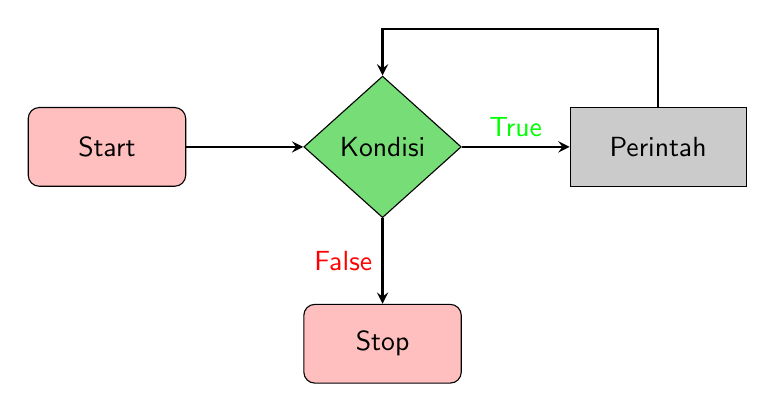
\begin{tikzpicture}
                \node (start) [startstop] {Start};
                \node (dec1) [decision, right of=start, xshift=2.5cm] {Kondisi};
                \node (pro1) [process, right of=dec1, xshift=2.5cm] {Perintah};
                \node (stop) [startstop, below of=dec1, yshift=-1.5cm] {Stop};

                \draw [arrow] (start) -- (dec1);
                \draw [arrow] (dec1) -- node[anchor=south] {\color{green}True} (pro1);
                \draw [arrow] (dec1) -- node[anchor=east] {\color{red}False} (stop);
                \draw [arrow] (pro1) -- ++(0,1.5) -| (dec1);
            \end{tikzpicture}
            \caption{Flowchart While}
        \end{figure}
    \end{frame}

    \begin{frame}[fragile]
        \frametitle{\insertsection}
        \begin{contoh}
            Program untuk menghentikan hacker yang sedang mencuri data warga negara.
        \end{contoh}
        \begin{lstlisting}
    int i = 1;
    boolean mencuri = true;
    while (mencuri) {
        System.out.println("Hacker jangan mencuri!");
        if (i == 3) {
            mencuri = false;
        } else {
            i++;
        }
    }
    System.out.println("Selamat data warga negara telah aman!");
        \end{lstlisting}
    \end{frame}

    \section{Do-While}
    \begin{frame}[fragile]
        \frametitle{\insertsection}
        \begin{definisi}
            \textbf{Do-While} adalah salah satu struktur pengulangan yang digunakan untuk melakukan sesuatu berulang kali. Struktur ini memiliki dua bagian, yaitu perintah dan kondisi. Struktur ini biasanya digunakan ketika kita ingin melakukan sesuatu minimal satu kali.
        \end{definisi}
        \begin{lstlisting}[caption={Syntax Do-While}, numbers=none]
    do {
        // Perintah yang akan diulang
    } while ("kondisi");
        \end{lstlisting}
    \end{frame}

    \begin{frame}
        \frametitle{\insertsection}
        \begin{figure}
            \centering
            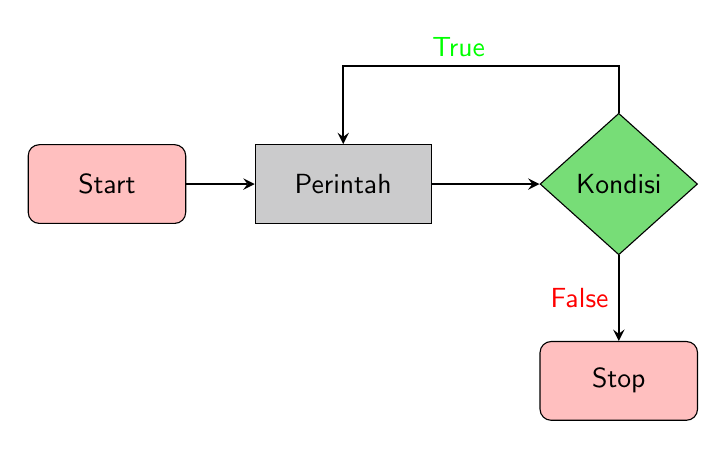
\begin{tikzpicture}
                \node (start) [startstop] {Start};
                \node (pro1) [process, right of=start, xshift=2cm] {Perintah};
                \node (dec1) [decision, right of=pro1, xshift=2.5cm] {Kondisi};
                \node (stop) [startstop, below of=dec1, yshift=-1.5cm] {Stop};

                \draw [arrow] (start) -- (pro1);
                \draw [arrow] (pro1) -- (dec1);
                \draw [arrow] (dec1) --  ++(0,1.5) -| node[anchor=north west,yshift=0.5cm,xshift=1cm] {\color{green}True} (pro1);
                \draw [arrow] (dec1) -- node[anchor=east] {\color{red}False} (stop);
            \end{tikzpicture}
            \caption{Flowchart Do-While}
        \end{figure}
    \end{frame}

    \begin{frame}
        \frametitle{\insertsection}
        \begin{alertblock}{Perbedaan}
            Perbedaan utama antara \textbf{While} dan \textbf{Do-While} adalah \textbf{While} melakukan pengecekan kondisi sebelum melakukan perintah, sedangkan \textbf{Do-While} melakukan perintah terlebih dahulu sebelum melakukan pengecekan kondisi. Jadi \textbf{Do-While} pasti akan melakukan perintah minimal satu kali.
        \end{alertblock}
    \end{frame}

    \begin{frame}[fragile]
        \frametitle{\insertsection}
        \begin{contoh}
            Countdown sebelum kuis.
        \end{contoh}
        \begin{lstlisting}[firstnumber=12]
    int hari = 4;
    boolean malas = true;
    do{
        System.out.println("Santai masih "+hari+" hari lagi");
        if (hari == 2) {
            malas = false;}
        hari--;
        }while(malas);
    System.out.println("Waduh besok udah kuis, ayo belajar!");
        \end{lstlisting}
    \end{frame}

    \section{Latihan}
    \begin{frame}
        \begin{latihan}
            Buatlah program untuk menampilkan barisan Fibonacci dengan input $n$ adalah banyaknya suku yang diinginkan.
        \end{latihan}
        \begin{funfact}
            Barisan Fibonacci juga bisa disebut Deret Fibonacci, padahal deret dan barisan merupakan dua hal yang berbeda. Ada yang tau alasannya?
        \end{funfact}
    \end{frame}
    
    \begin{frame}[fragile]
        \begin{latihan}
            Buatlah program for-loop yang masing-masing menampilkan pola berikut:
        \end{latihan}
        \begin{columns}
            \begin{column}{0.3\textwidth}
                \begin{lstlisting}[style=output]
    
           *
          ***
         *****
        *******
       *********
       (**)
                \end{lstlisting}
            \end{column}
            \begin{column}{0.3\textwidth}
                \begin{lstlisting}[style=output]
    
        *********
       *       *
      *       *
     *       *
    *********
    (**)
                \end{lstlisting}
            \end{column}
            \begin{column}{0.3\textwidth}
                \begin{lstlisting}[style=output]
        **   **
       **** ****
       *********
        *******
         *****
          ***
           *
                \end{lstlisting}
            \end{column}
        \end{columns}
    \end{frame}
\end{document}